\section{Panel multi-activo: rescate pareado, agregado y por régimen}
\label{sec:mp-panel}

% Fuente única de cifras: notebooks/STRATA_marco_practico.ipynb (panel canónico de 10) y sus JSON en
% outputs/experiments/. Toda cifra trazada a su JSON en el caption de su tabla.

SPY enseña el mecanismo, pero un activo no prueba nada. La prueba dura vive en el panel: diez activos (SPY, QQQ, XLF, DIA, XLK, XLE, ROKU, SMCI, MARA, UNG), elegidos por su naturaleza para cubrir distintos grados de \emph{leverage effect}. Sobre ellos repetimos toda la cadena de SPY y agregamos los resultados. Aquí está el resultado central del capítulo: el rescate de riesgo, que en un activo cruzaba el cero, alcanza significancia al apilar el panel.

\subsection{El agente en el panel y la activación de detectores}
\label{sec:mp-panel-agente}

El problema que vimos en SPY no es de SPY. A través del panel el agente pierde y acierta menos de la mitad de las direcciones con regularidad: su accuracy va de $0{,}366$ en SPY a $0{,}528$ en MARA, y queda por debajo de $0{,}5$ en siete de los diez activos. Allí donde supera el medio punto lo hace por poco, y su Sharpe sigue siendo pobre. El agente solo no es una estrategia, es el punto de partida que STRATA tiene que corregir.

Los tres detectores no se encienden por igual en cada activo. RAM domina en todas partes, igual que en SPY: es el canal que lee el régimen y el que carga con el rescate. PSA y GSO disparan poco, porque el agente mantiene posiciones casi constantes y sus \emph{scores} de cambio y de tamaño rara vez cruzan los umbrales de calibración. La Tabla~\ref{tab:mp-gate} recoge la tasa de intervención por activo y la compuerta de régimen. El gate RAM es la lectura que importa: en los días en que RAM dispara, seguir el signo del régimen bate a seguir al agente en \textbf{seis de los diez} activos. La intervención no se reparte al azar. Su tasa crece con la discrepancia entre la apuesta del agente y el signo del régimen, y esa relación es casi recta: la correlación de Pearson entre discrepancia y tasa de intervención es $r = 0{,}93$ con $p < 0{,}001$.

\begin{table}[htbp]
\centering
\caption{Activación de RAM y compuerta de régimen por activo (OOS completo del panel). ``Tasa interv.'' es la fracción de días en que RAM dispara; ``discrepancia'' es la fracción de días en que la apuesta del agente choca con el signo del régimen; ``gate RAM'' indica si, en los días de disparo, seguir el régimen bate a seguir al agente. PSA y GSO disparan de forma marginal en todo el panel. Fuente: \texttt{spy\_panel\_gate\_descriptive.json}, \texttt{mechanism\_panel.json}.}
\label{tab:mp-gate}
\begin{tabular}{lrrl}
\toprule
Activo & Tasa interv.\ (RAM) & Discrepancia agente$\leftrightarrow$régimen & Gate RAM \\
\midrule
SPY  & $0{,}302$ & $0{,}601$ & régimen $>$ agente \\
QQQ  & $0{,}197$ & $0{,}526$ & régimen $>$ agente \\
XLF  & $0{,}549$ & $0{,}720$ & régimen $>$ agente \\
DIA  & $0{,}343$ & $0{,}603$ & agente $>$ régimen \\
XLK  & $0{,}095$ & $0{,}372$ & agente $>$ régimen \\
XLE  & $0{,}596$ & $0{,}781$ & régimen $>$ agente \\
ROKU & $0{,}710$ & $0{,}823$ & régimen $>$ agente \\
SMCI & $0{,}018$ & $0{,}120$ & régimen $>$ agente \\
MARA & $0{,}415$ & $0{,}666$ & agente $>$ régimen \\
UNG  & $0{,}078$ & $0{,}169$ & agente $>$ régimen \\
\bottomrule
\end{tabular}
\end{table}

\begin{figure}[htbp]
\centering
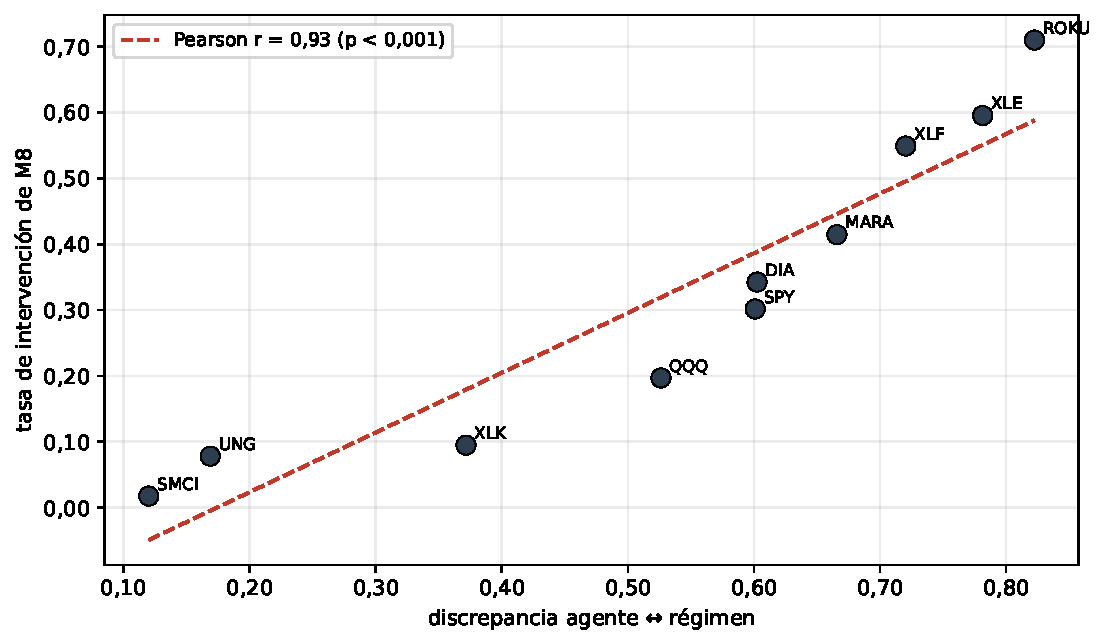
\includegraphics[width=0.85\textwidth]{figuras/cap4_gate_ram}
\caption{Compuerta de régimen sobre el panel: tasa de intervención de RAM frente a la discrepancia media entre la apuesta del agente y el signo del régimen, un punto por activo. La relación es casi recta (Pearson $r = 0{,}93$, $p < 0{,}001$): cuanto más se aleja el agente del estado del mercado, con más frecuencia actúa la regla. Fuente: \texttt{spy\_panel\_gate\_descriptive.json}.}
\label{fig:mp-gate-ram}
\end{figure}

La compuerta gobierna toda la lectura del panel. RAM deja pasar la decisión del agente salvo cuando choca con el régimen, y solo entonces la corrige; en seis de los diez activos esa corrección apunta en la dirección buena. Que la actividad de la regla escale con la discrepancia es la prueba de que la intervención no es indiscriminada: trabaja donde el agente y el mercado de verdad se contradicen, y se calla donde ya coinciden.

\subsection{Accuracy por activo y estrategia: dónde se bate a la trivial}
\label{sec:mp-panel-tabla}

La Tabla~\ref{tab:mp-accuracy} cruza los diez activos con las seis estrategias en accuracy direccional. La primera lectura es contundente: la mejor derivada de STRATA mejora al agente en los \textbf{diez de diez} activos, con una mejora media de accuracy de $+0{,}086$. No hay ningún activo en el que supervisar al agente lo empeore. Qué estrategia gana cambia de un activo a otro, y eso es coherente con la idea de dos capas: en unos manda la regla, en otros el aprendiz, según la naturaleza del activo.

\begin{table}[htbp]
\centering
\caption{Accuracy direccional por activo y estrategia (ventana desplegable, \texttt{signal\_lag}${}=1$). En negrita, la mejor derivada de STRATA (M8/M10/AutoML) cuando supera a las dos referencias triviales (ZeroR y B\&H) en ese activo. ZeroR y B\&H comparten valor salvo cuando difieren. Fuente: \texttt{automl\_runs/panel\_mm25\_inclGBM-XGB-SE\_AUC\_emb1\_N0-150\_step21\_kfold\_seed42.json}.}
\label{tab:mp-accuracy}
\begin{tabular}{lrrrrrr}
\toprule
Activo & M5 & M8 & M10 & AutoML & ZeroR & B\&H \\
\midrule
SPY  & $0{,}366$ & $0{,}442$ & $0{,}494$ & $\mathbf{0{,}574}$ & $0{,}566$ & $0{,}566$ \\
QQQ  & $0{,}418$ & $0{,}486$ & $0{,}522$ & $0{,}534$ & $0{,}590$ & $0{,}590$ \\
XLF  & $0{,}429$ & $0{,}502$ & $0{,}526$ & $0{,}510$ & $0{,}539$ & $0{,}539$ \\
DIA  & $0{,}440$ & $0{,}484$ & $0{,}468$ & $0{,}520$ & $0{,}552$ & $0{,}556$ \\
XLK  & $0{,}510$ & $0{,}470$ & $0{,}542$ & $0{,}590$ & $0{,}641$ & $0{,}641$ \\
XLE  & $0{,}448$ & $0{,}528$ & $0{,}508$ & $0{,}532$ & $0{,}565$ & $0{,}565$ \\
ROKU & $0{,}444$ & $0{,}528$ & $0{,}508$ & $0{,}544$ & $0{,}548$ & $0{,}548$ \\
SMCI & $0{,}484$ & $0{,}496$ & $\mathbf{0{,}552}$ & $0{,}472$ & $0{,}516$ & $0{,}484$ \\
MARA & $0{,}528$ & $0{,}528$ & $0{,}532$ & $\mathbf{0{,}544}$ & $0{,}532$ & $0{,}468$ \\
UNG  & $0{,}510$ & $0{,}502$ & $\mathbf{0{,}518}$ & $0{,}482$ & $0{,}449$ & $0{,}486$ \\
\bottomrule
\end{tabular}
\end{table}

Hay cuatro activos en los que una derivada de STRATA supera en punto a las dos referencias triviales a la vez. En SPY, AutoML alcanza $0{,}574$ frente a $0{,}566$ del pasivo. En SMCI, M10 llega a $0{,}552$, por encima de $0{,}516$ de ZeroR y $0{,}484$ de B\&H. En MARA, AutoML acierta $0{,}544$ contra $0{,}532$ y $0{,}468$. En UNG, M10 logra $0{,}518$ frente a $0{,}449$ y $0{,}486$. En los seis activos restantes la trivial aguanta: en índices muy direccionales como XLK la clase mayoritaria del pasado acierta $0{,}641$, y ninguna derivada se le acerca.

Estas victorias son reales en punto y conviene leerlas con cuidado. Son nominales: la ventana desplegable tiene del orden de doscientos cincuenta días por activo, y la estrategia ganadora cambia de un activo a otro, de modo que se eligen a posteriori. \textbf{Ninguna bate a ZeroR con significancia}: el McNemar pareado de AutoML frente a ZeroR sobre SPY da $p = 0{,}90$, sin potencia para separarlos. Reportamos el punto porque es parte del valor, y marcamos el límite porque no sobrevive a un test. La Figura~\ref{fig:mp-heatmap} hace visible el mapa completo: el color mide la distancia a la trivial, y solo cuatro celdas de derivada se tiñen del lado bueno.

\begin{figure}[htbp]
\centering
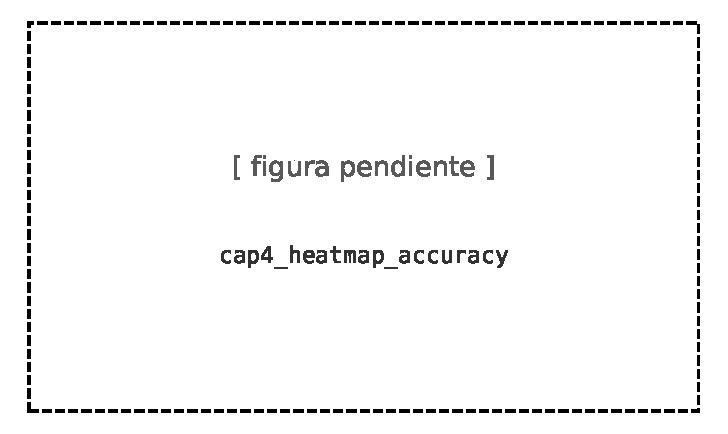
\includegraphics[width=0.9\textwidth]{figuras/cap4_heatmap_accuracy}
\caption{Mapa de calor de la accuracy direccional por activo (filas) y estrategia (columnas), centrado en $0{,}5$: el color mide la distancia a una referencia trivial. Verde marca accuracy por encima de la trivial del activo, rojo por debajo. La mejor derivada de STRATA supera a las dos triviales solo en SPY, SMCI, MARA y UNG; en los demás la trivial aguanta. Victorias nominales (n${}\approx 250$, a posteriori; McNemar AutoML vs ZeroR en SPY $p = 0{,}90$). Fuente: \texttt{automl\_runs/panel\_mm25\_inclGBM-XGB-SE\_AUC\_emb1\_N0-150\_step21\_kfold\_seed42.json}.}
\label{fig:mp-heatmap}
\end{figure}

La accuracy deja una conclusión clara y un límite honesto. STRATA rescata al agente en los diez activos, y en cuatro la derivada le gana en punto a las dos referencias triviales, sobre todo en los de \emph{leverage} débil o invertido. Pero la ventaja sobre la trivial es nominal, no significativa, y la ganadora no es la misma en todas partes. La prueba que sí sobrevive a un test no está en la accuracy frente a la trivial: está en el riesgo, y la damos a continuación.

\subsection{Pooled-10: el rescate en riesgo}
\label{sec:mp-panel-riesgo}

Este es el resultado duro del capítulo. Sobre un único activo, el intervalo de confianza del $\Delta$Sharpe del rescate frente al agente cruzaba el cero; lo anunciamos al cerrar SPY. La solución es agregar: apilamos los días de los diez activos (\emph{pooled-10}, $n = 2493$ días) y medimos el $\Delta$Sharpe pareado frente a M5 con un \emph{bootstrap} estacionario de bloque medio $\sqrt{n}$ (Politis y Romano 1994 \cite{politis1994}), que respeta la dependencia temporal de las series. La Tabla~\ref{tab:mp-pooled} reúne las tres estrategias supervisadas.

Las tres rescatan al agente en riesgo, y las tres excluyen el cero. La regla M8 deja un $\Delta$Sharpe de $+0{,}60$ con intervalo $[0{,}05,\ 1{,}22]$. El meta-learner M10 sube a $+1{,}12$ con $[0{,}39,\ 1{,}84]$. AutoML alcanza $+1{,}08$ con $[0{,}40,\ 1{,}85]$. Que el límite inferior del intervalo quede por encima de cero es la afirmación que el caso SPY no podía sostener en solitario: el rescate de riesgo es estadísticamente distinguible de cero sobre el panel.

\begin{table}[htbp]
\centering
\caption{Rescate en riesgo agregado (\emph{pooled-10}, $n = 2493$ días): $\Delta$Sharpe de cada estrategia supervisada frente al agente M5, con intervalo de confianza al $95\,\%$ por \emph{bootstrap} estacionario de bloque medio $\sqrt{n}$ (Politis y Romano 1994). La columna de Bonferroni aplica la cota inferior corregida por $m = 3$ comparaciones (López de Prado 2018): un $\Delta$Sharpe pasa si su cota inferior corregida supera cero. M10 y AutoML pasan; M8 no. Fuente: \texttt{bullbear\_confirmatory.json} (bloque \texttt{POOLED10}).}
\label{tab:mp-pooled}
\begin{tabular}{lrcrc}
\toprule
Estrategia & $\Delta$Sharpe & IC$_{95}$ & Cota inf.\ Bonferroni & ¿Pasa? \\
\midrule
M8 (regla)            & $+0{,}60$ & $[0{,}05,\ 1{,}22]$ & $-0{,}047$ & no \\
M10 (meta-learner)    & $+1{,}12$ & $[0{,}39,\ 1{,}84]$ & $+0{,}258$ & sí \\
\textbf{AutoML} (H2O) & $\mathbf{+1{,}08}$ & $[0{,}40,\ 1{,}85]$ & $\mathbf{+0{,}261}$ & sí \\
\bottomrule
\end{tabular}
\end{table}

La corrección por multiplicidad mete un matiz que no escondemos. Comparamos tres estrategias contra el mismo agente, así que el intervalo de cada una debe corregirse por las $m = 3$ pruebas para no inflar la confianza (López de Prado 2018 \cite{lopezdeprado2018}). Bajo la cota de Bonferroni, M10 y AutoML siguen pasando, con cota inferior de $+0{,}258$ y $+0{,}261$. La regla M8 no pasa: su cota inferior corregida cae a $-0{,}047$, justo por debajo de cero. Es una falsación honesta. La regla rescata el riesgo en punto y con intervalo simple, pero su ventaja no sobrevive a la corrección por número de pruebas; los aprendices sí. La Figura~\ref{fig:mp-forest} lo dibuja: M8 toca el cero bajo Bonferroni mientras M10 y AutoML se mantienen del lado bueno.

\begin{figure}[htbp]
\centering
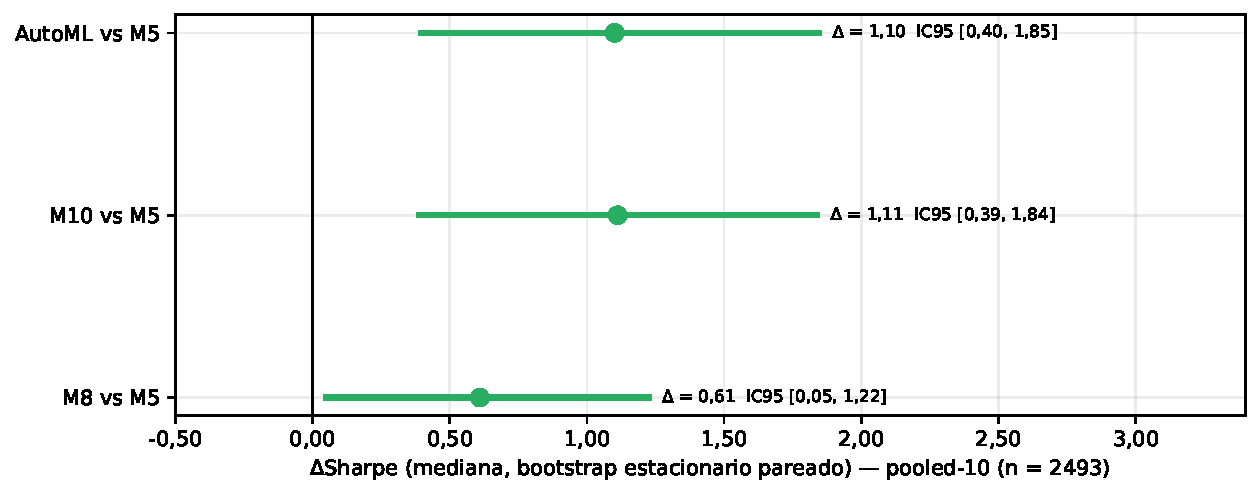
\includegraphics[width=0.85\textwidth]{figuras/cap4_forest_pooled}
\caption{Diagrama de bosque del $\Delta$Sharpe \emph{pooled-10} frente al agente M5, con intervalo al $95\,\%$ (\emph{bootstrap} estacionario, Politis y Romano 1994) y cota inferior corregida por Bonferroni ($m = 3$). La línea vertical marca el cero. Los tres intervalos simples excluyen el cero; bajo Bonferroni, M10 y AutoML se mantienen positivos y M8 toca el cero (cota inferior $-0{,}047$). Fuente: \texttt{bullbear\_confirmatory.json} (bloque \texttt{POOLED10}).}
\label{fig:mp-forest}
\end{figure}

Una cautela sobre el agregado, que es propia del método y la declaramos. El \emph{pooled} apila los días de los diez activos como si fueran independientes, y no lo son: la correlación cruzada entre índices es alta, con SPY y QQQ por encima de $0{,}9$. Eso reduce el tamaño de muestra efectivo por debajo del nominal y deja el intervalo algo optimista. El bloque medio $\sqrt{n}$ del \emph{bootstrap} amortigua parte del efecto, porque remuestrea bloques contiguos en lugar de días sueltos, pero el intervalo \emph{pooled} debe leerse con esa cautela. Aun así, el $+0{,}60$ de M8 excluye el cero en el intervalo simple, y los aprendices lo hacen también bajo Bonferroni.

La Figura~\ref{fig:mp-equity-panel} traslada el riesgo a la economía, una curva de capital por activo con la ganadora destacada. En cuatro activos una derivada de STRATA bate al pasivo en Sharpe: SPY, SMCI, MARA y UNG. La lectura razonada separa dos casos. En SMCI, MARA y UNG el pasivo pierde o ronda el cero, y la derivada saca un Sharpe positivo claro yendo defensiva en el momento bueno: ahí la ventaja parece valor direccional, porque no viene de estar largo en una subida. En SPY la cosa es distinta. El periodo fue alcista y SPY es mayormente beta de mercado, así que el Sharpe positivo refleja sobre todo la exposición al índice más que una dirección acertada. Distinguir las dos cosas exige un contraste que no hacemos aquí; queda como lectura, no como afirmación.

\begin{figure}[htbp]
\centering
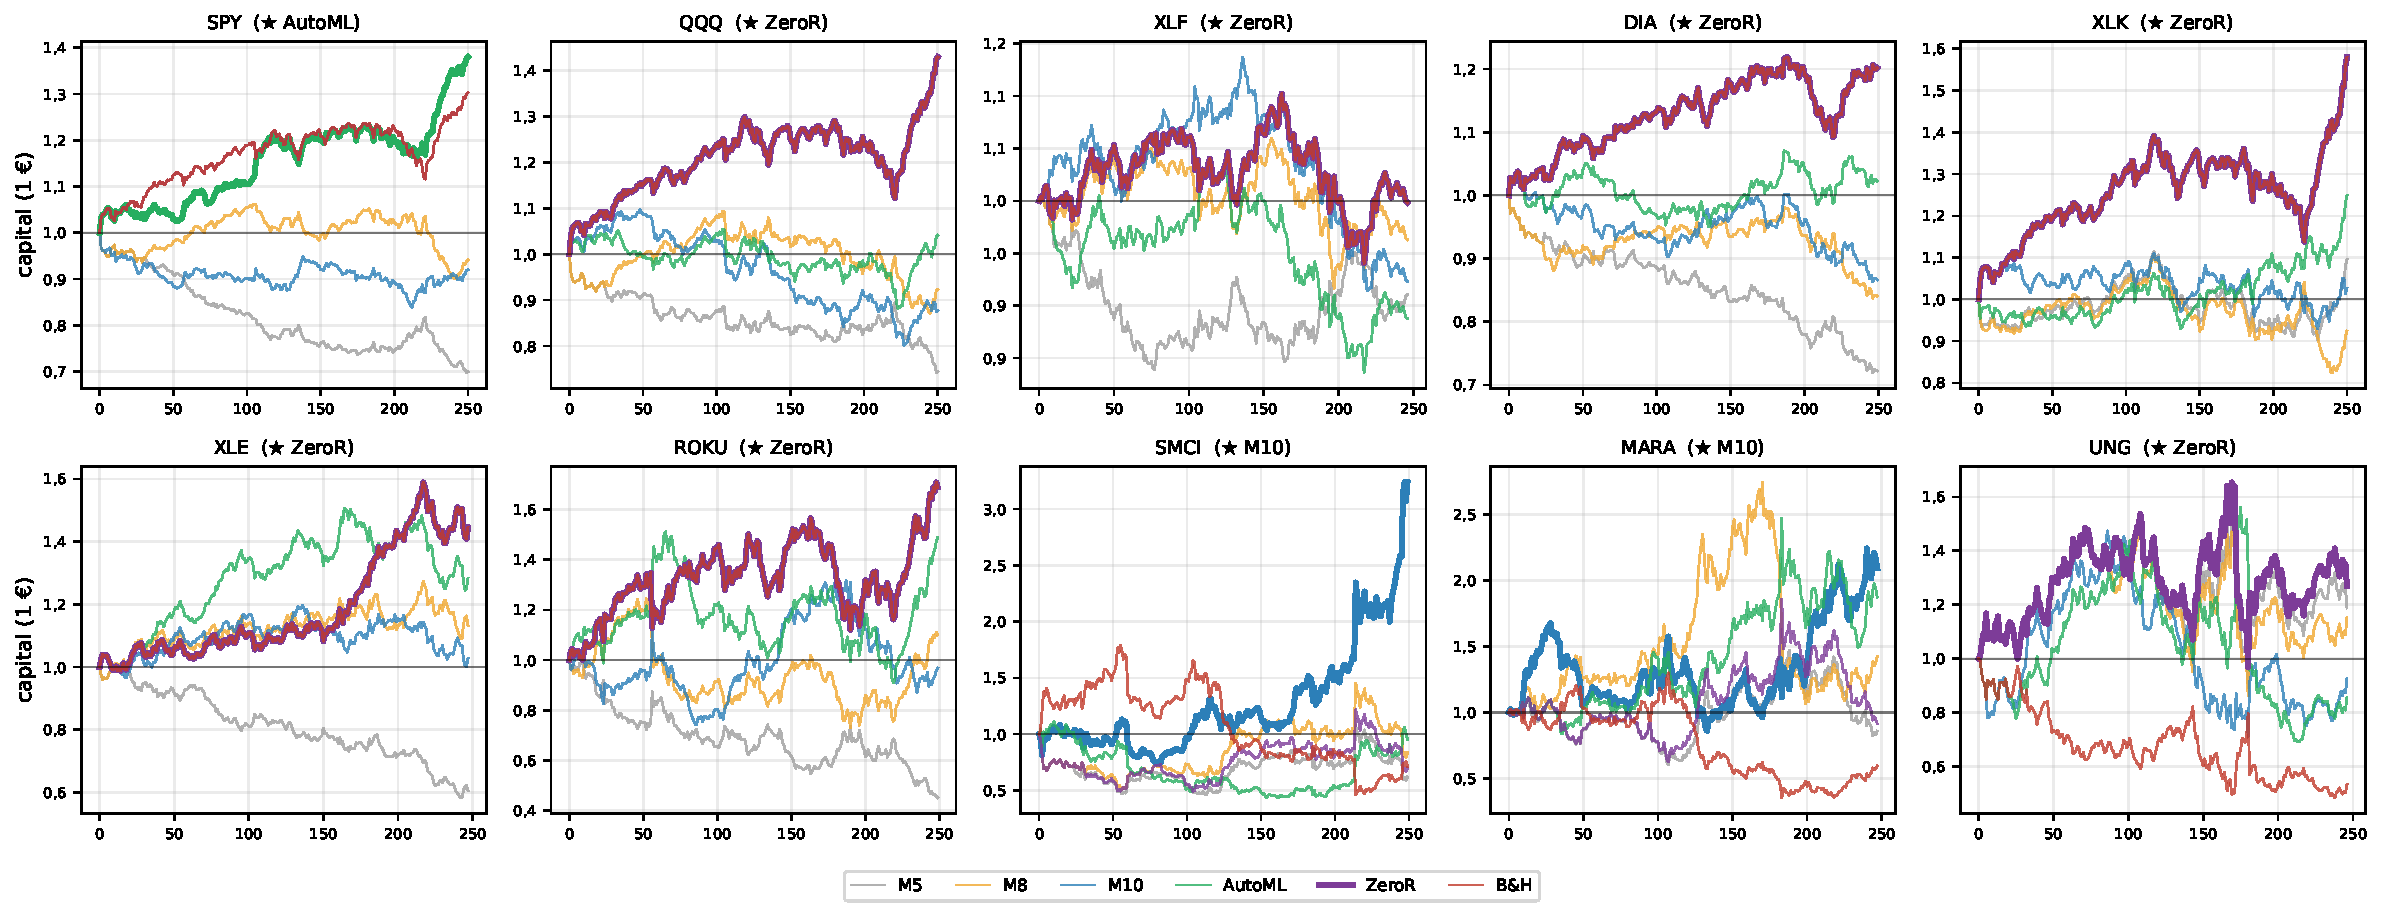
\includegraphics[width=0.95\textwidth]{figuras/cap4_equity_panel}
\caption{Curvas de capital por activo (un euro inicial), con la mejor derivada de STRATA destacada frente a las referencias. En cuatro activos una derivada bate al pasivo en Sharpe: SPY, SMCI, MARA y UNG. En SMCI/MARA/UNG el pasivo pierde o ronda el cero y la derivada saca Sharpe positivo yendo defensiva (lectura de valor direccional); en SPY la ventaja es sobre todo beta de mercado en un periodo alcista. Lectura sin contraste asociado. Fuente: \texttt{automl\_net\_returns.json}.}
\label{fig:mp-equity-panel}
\end{figure}

\subsection{El aprendiz redescubre STRATA y bate a la regla}
\label{sec:mp-panel-tost}

Si el aprendiz mejora a la regla, la pregunta es de qué se está alimentando. La respuesta es que se apoya en los detectores de STRATA. Las cuotas de Shapley (Lundberg y Lee 2017 \cite{lundberg2017}) miden cuánto del juicio del aprendiz descansa en cada bloque de características; la cuota de las features de STRATA supera la mitad en los \textbf{diez de diez} activos, con una media de $0{,}66$. El aprendiz no inventa una señal nueva: redescubre los detectores que diseñamos a mano y los pondera por encima de las características del propio agente.

Que se apoye en STRATA no quiere decir que solo replique la regla. El contraste lo da el TOST, el doble test unilateral de equivalencia (Schuirmann 1987 \cite{schuirmann1987}), que pregunta si dos estrategias son indistinguibles dentro de un margen. La Tabla~\ref{tab:mp-tost} lo aplica al aprendiz frente a la regla M8. En accuracy no hay equivalencia, y el desempate va para el aprendiz: M10 supera a la regla en $+0{,}021$ con intervalo al $90\,\%$ de $[+0{,}001,\ +0{,}039]$, y AutoML en $+0{,}034$ con $[+0{,}010,\ +0{,}056]$. En Sharpe el TOST es no concluyente: aprendiz y regla son indistinguibles en riesgo, ninguno domina al otro. El mecanismo de la diferencia es claro. La regla M8 es una compuerta fija sobre el régimen; el aprendiz modela interacciones no lineales entre régimen y agente que la regla no alcanza, y de ahí saca el punto extra de accuracy.

\begin{table}[htbp]
\centering
\caption{TOST del aprendiz frente a la regla M8 (Schuirmann 1987) y cuota de Shapley de las features de STRATA por activo (Lundberg y Lee 2017). En accuracy el aprendiz supera a la regla (intervalo al $90\,\%$ por encima de cero); en Sharpe el test es no concluyente (indistinguibles). La cuota SHAP de STRATA supera $0{,}5$ en los diez activos. Fuente: \texttt{equivalence\_tost.json}, \texttt{decision\_automl\_prep.json}.}
\label{tab:mp-tost}
\begin{tabular}{lccc}
\toprule
Comparación & $\Delta$accuracy (IC$_{90}$) & TOST Sharpe & Cuota SHAP STRATA \\
\midrule
M10 vs M8     & $+0{,}021\ [+0{,}001,\ +0{,}039]$ & no concluyente & \multirow{2}{*}{$>0{,}5$ en $10/10$ (media $0{,}66$)} \\
AutoML vs M8  & $+0{,}034\ [+0{,}010,\ +0{,}056]$ & no concluyente & \\
\bottomrule
\end{tabular}
\end{table}

\begin{figure}[htbp]
\centering
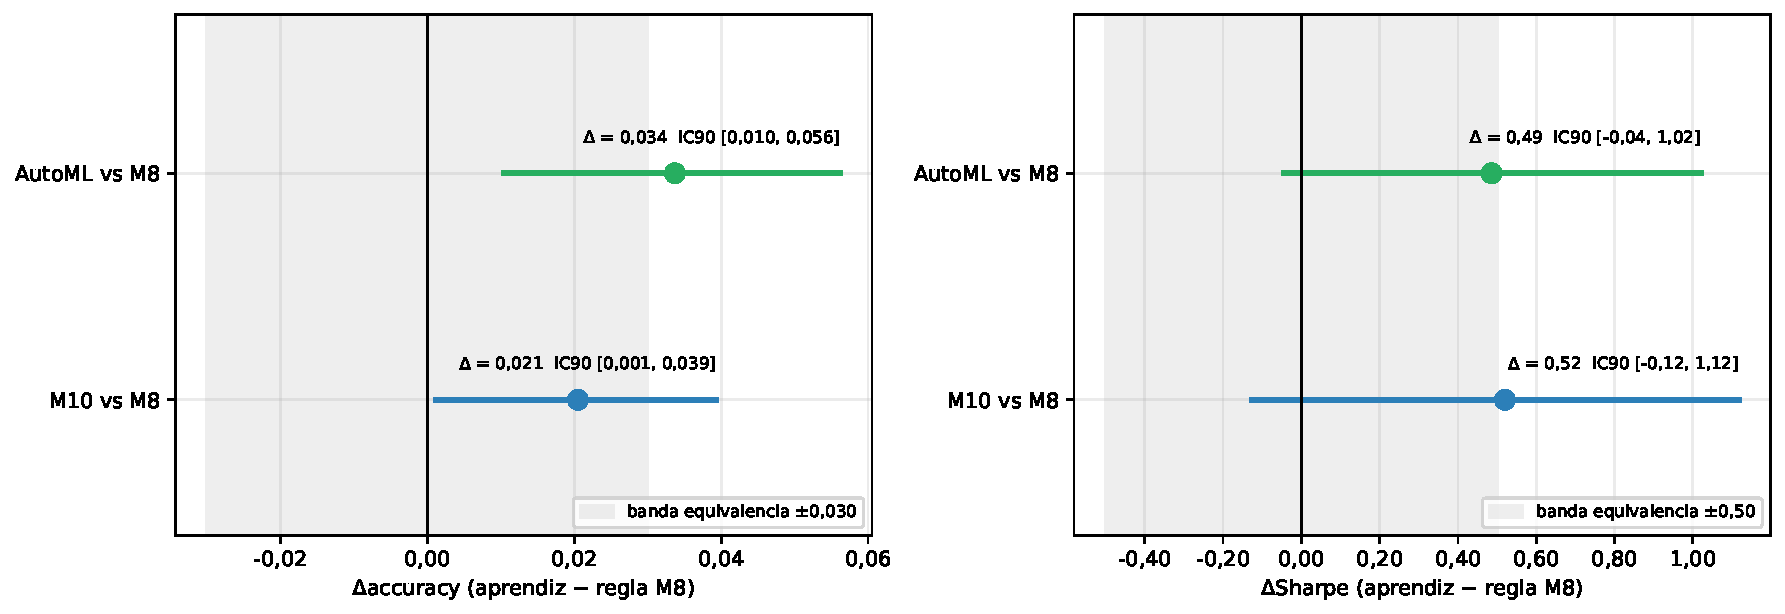
\includegraphics[width=0.8\textwidth]{figuras/cap4_tost_2x2}
\caption{Diagrama $2\times 2$ del TOST del aprendiz frente a la regla M8, ejes accuracy (horizontal) y Sharpe (vertical). Las regiones marcan superioridad, equivalencia y no concluyencia. M10 y AutoML caen en superioridad en accuracy y en no concluyencia en Sharpe: el aprendiz afina la dirección sobre la regla y empata en riesgo. Fuente: \texttt{equivalence\_tost.json}.}
\label{fig:mp-tost}
\end{figure}

El aprendiz deja, entonces, dos hechos atados con su test. Se apoya en STRATA, con cuota SHAP mayoritaria en los diez activos, lo que descarta que gane por otro lado. Y bate modestamente a la regla en accuracy sin distinguirse de ella en riesgo. La regla protege el riesgo, el aprendiz afina la dirección apoyándose en las mismas señales.

\subsection{Robustez por régimen: bull, bear y complementariedad}
\label{sec:mp-panel-regimen}

Un rescate que solo funcionara en mercado alcista no serviría de mucho, porque el régimen peligroso es el bajista. Partimos el panel por régimen y medimos el rescate en cada mitad con el McNemar pooled de la estrategia superior frente al agente, corrigiendo por Holm las comparaciones múltiples (Holm 1979 \cite{holm1979}). El rescate aparece en los dos regímenes. En alcista, M10 da $p = 0{,}0076$ y AutoML $p = 0{,}0092$, ambos significativos; la regla M8 queda al borde, con $p = 0{,}099$. En bajista, M8 alcanza $p = 0{,}0092$, M10 $p = 0{,}0268$ y AutoML $p = 0{,}0017$. El rescate no es de un solo régimen: sobrevive en los dos.

\begin{table}[htbp]
\centering
\caption{Rescate por régimen (McNemar pooled de la estrategia superior frente a M5, $p$ corregido por Holm 1979) y complementariedad de los aprendices (DiD). El rescate es significativo en alcista y en bajista. El DiD contrasta el $\Delta\Delta$Sharpe entre aprendices y regímenes: M10 rescata más en alcista, AutoML más en bajista. Fuente: \texttt{bullbear\_confirmatory.json}, \texttt{regime\_did\_learners.json}.}
\label{tab:mp-regimen}
\begin{tabular}{lccc}
\toprule
 & M8 & M10 & AutoML \\
\midrule
McNemar alcista (Holm $p$) & $0{,}099$ & $0{,}0076$ & $0{,}0092$ \\
McNemar bajista (Holm $p$) & $0{,}0092$ & $0{,}0268$ & $0{,}0017$ \\
\midrule
\multicolumn{4}{l}{DiD complementariedad: $\Delta\Delta$Sharpe pooled $= +1{,}37$, IC$_{95}\,[0{,}20,\ 2{,}60]$, $p = 0{,}008$} \\
\bottomrule
\end{tabular}
\end{table}

Los dos aprendices no rescatan igual en cada régimen, y eso abre una vía. M10 protege más en alcista, AutoML más en bajista. Para contrastar si ese reparto es real y no ruido construimos un test de diferencia-en-diferencias, pre-registrado antes de mirar resultados: comparamos la diferencia de $\Delta$Sharpe entre los dos aprendices entre los dos regímenes, de modo que cualquier efecto común a ambos se cancela y queda solo la complementariedad. El $\Delta\Delta$Sharpe pooled es $+1{,}37$ con intervalo $[0{,}20,\ 2{,}60]$ y $p = 0{,}008$, que excluye el cero. La complementariedad por régimen es significativa sobre el panel. La Figura~\ref{fig:mp-did} la dibuja: AutoML cubre el régimen peligroso, M10 el favorable.

\begin{figure}[htbp]
\centering
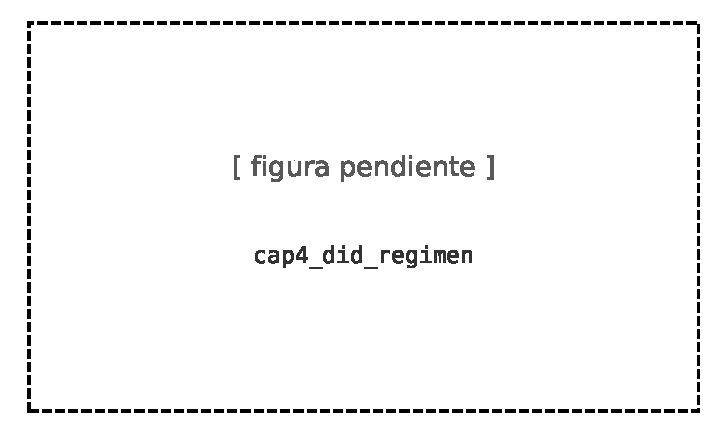
\includegraphics[width=0.8\textwidth]{figuras/cap4_did_regimen}
\caption{Complementariedad de los aprendices por régimen: $\Delta$Sharpe de M10 y de AutoML frente al agente, en alcista y en bajista. M10 rescata más en alcista, AutoML más en bajista; el contraste de diferencia-en-diferencias del reparto da $\Delta\Delta$Sharpe $= +1{,}37$, IC$_{95}\,[0{,}20,\ 2{,}60]$, $p = 0{,}008$ (pooled; no significativo en SPY solo). Fuente: \texttt{regime\_did\_learners.json}.}
\label{fig:mp-did}
\end{figure}

Conviene cerrar con la falsación que pre-registramos y que el panel resuelve. A nivel de SPY solo, en régimen bajista la regla M8 se invierte: sobre los cincuenta días bajistas de SPY su $\Delta$Sharpe es $-1{,}49$, es decir, ahí la regla daña en vez de rescatar. Es exactamente el tipo de fragilidad que un activo único puede esconder o magnificar con cincuenta observaciones. La agregación del panel la resuelve: sobre los diez activos el rescate por régimen es significativo en bajista, y la complementariedad DiD también lo es solo en \emph{pooled}, no en SPY aislado. El fenómeno es de panel, no de un activo, y por eso la prueba vive en la agregación.

Agregado el panel, el rescate deja de ser una anécdota de SPY. En riesgo es significativo: el $\Delta$Sharpe \emph{pooled-10} excluye el cero para los tres modelos, y dos de los tres sobreviven a Bonferroni. En accuracy el aprendiz rescata al agente en los diez activos y bate modestamente a la regla, apoyándose en las señales de STRATA con cuota SHAP mayoritaria. Las dos capas se reparten el trabajo: la regla protege el riesgo, el aprendiz afina la dirección, y los aprendices se complementan por régimen. Queda una pregunta abierta, el porqué del reparto por activo, por qué unos se rescatan por régimen y otros por el aprendiz. Eso lo explica la naturaleza del activo, y es lo que aborda la Sección~\ref{sec:mp-mecanismo}.
